\chapter{Discipline: nulls, simulations, pre-registration}\label{ch:discipline}

\section{Why an instrument needs rules about itself}

A methylome offers hundreds of thousands of places to find a pattern and dozens of choices at every step of an analysis. Cosmology learned, at
cost, that a result is only as good as the discipline that produced it: pre-registered tests, null tests that must read zero, simulations that must
recover what was put in, and a correction for every place one looked. The chain adopts all four, and one more that cosmology takes for granted: the
record of how every number was obtained is kept with the number. The record of how a result was obtained is as important as the result.

\section{Pre-registration}

A procedure that decides anything about the instrument is written before data are read: what is built, what is measured, the bars it must meet, and what
each outcome decides. It is committed to the repository with a timestamp, and its SHA is quoted in the outcome. The outcome is scored against the bars as
written; nothing moves after results are visible. A bar that fails is recorded as failed, with a diagnostic written after the bars and labelled as such.
An error found in a pre-registration is recorded first in the outcome and the pre-registration is left unchanged.

Three refinements came from use.
\begin{itemize}
\item \textbf{A deferred check is never a pass.} A gate that cannot run because an input is missing stops the specimen (Chapter~\ref{ch:instrument}).
\item \textbf{Development and commissioning are different stages.} During development the chain is diagnosed, fixed and re-run as often as needed, and each
      result is reported and marked \emph{development, after looking}. Pre-registration governs the procedures that commission the instrument and produce
      evidence. Chain v3 is a development build; no cell is commissioned.
\item \textbf{A pass must survive the obvious confound.} In one pre-registered battery, severe infection read above Normal more often than health
      (one-sided $p=0.015$), a pass as written. Severe specimens also had more neutrophils (median fraction 0.79 against 0.65), and with fraction in the model
      the severity term was $+0.0075$ ($p=0.42$). \measured{} The pass was a composition effect, and the
      outcome says so. The pre-registration had named that risk.
\end{itemize}

\section{Null tests}

\begin{center}\small
\begin{tabular}{@{}p{0.34\textwidth}p{0.36\textwidth}p{0.2\textwidth}@{}}\toprule
null & what must happen & chain v3 \\\midrule
held-out reference arrays & read Normal on sites and a floor chosen without them & 6 of 6; SD 0.020 \\
tared mixtures and remission bloods & read Normal & in Normal, each tared against the other specimens of its group, not against healthy references \\
same person, repeat draws & differences inside the change floor & floor not yet measured \\
technical replicates & differences inside the change floor & being measured in development \\
known mixtures of purified cells & fractions within the stated error & median 0.034 \\
inactive look-alike compound & no change & 1.002--1.032 \\\bottomrule
\end{tabular}
\end{center}
\measured{} The records behind each row are listed in the SOP.

Figure~\ref{fig:p4_nulls} shows every reading behind the table.

\begin{figure}[htbp]\centering
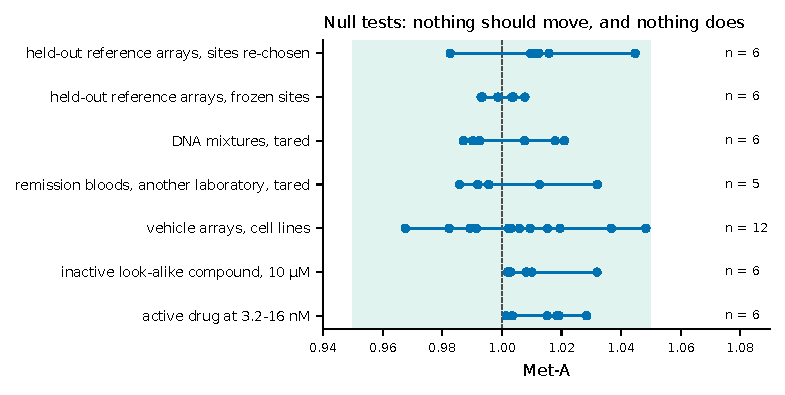
\includegraphics[width=0.62\textwidth]{figures/part6/fig_p4_18_nulls.pdf}
\caption{Null tests of chain v3, every reading. Held-out reference arrays; tared mixtures and remission bloods (acceptance run);
vehicle arrays, the inactive analogue and the two lowest doses of the active drug, each line against its own
vehicle (GSE135205~\cite{Pappalardi2021}). Normal shaded. \measured}
\label{fig:p4_nulls}
\end{figure}

\section{Constructed specimens and known causes}

A constructed specimen has a known change planted in it. Chain v3 computes one on every whole-blood reading: the shift a 1~\% loss of the neutrophil pattern
would cause at this specimen's own fraction, which sets its detection limit. On six known mixtures, a planted 2~\% loss moved the tared reading by $+0.061$
and above 1.05 on 6 of 6. \measured{} A planted change tests the arithmetic, not the biology. The stronger test is a
known physical cause: a DNA-methyltransferase inhibitor, an inactive analogue, and a dose series, read on arrays and on single molecules. The construction also found the entropy ceiling: past $\beta=\tfrac12$ further loss lowers $H$, so the chain prints the
methylated sites' mean $\beta$ beside every reading and flags a specimen past the ceiling.

Figure~\ref{fig:p4_planted} shows the planted loss on the six mixtures before any tare, with the fraction held and with it re-fitted.

\begin{figure}[htbp]\centering
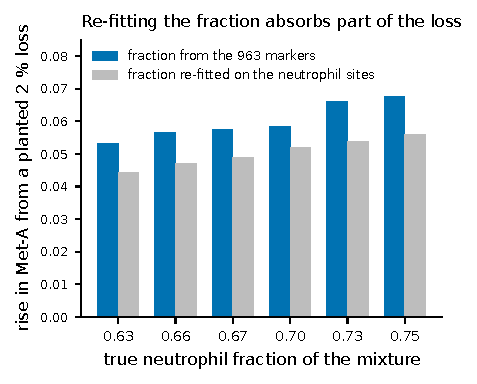
\includegraphics[width=0.5\textwidth]{figures/part6/fig_p4_18_planted.pdf}
\caption{Rise in untared whole-blood Met-A from a planted 2~\% loss of the neutrophil pattern, on the six mixtures with at least 50~\% neutrophils.
Fraction from the composition markers: 0.053--0.067. Fraction re-fitted on the neutrophil sites: 0.044--0.056; the fit takes up
part of the loss as a change of fraction. \measured}
\label{fig:p4_planted}
\end{figure}

\section{Look-elsewhere}

A search over many places must be corrected for the number of places. Chain v3 reads one statistic per cell per specimen, Met-A, and one map statistic, the
C-score, each defined before any specimen is read, so a reading involves no search. A comparison across many specimens, many sites or many lead times is a
search, and it carries the correction. Most patterns found by looking are the product of looking.


\section{Guards that run at every change}

A single build script regenerates the documents derived from the code and runs gates that include a vocabulary scan
that fails on condition names and group-comparison language in live text, a link check, and a reconciliation of each generated procedure with its source.
The chain v3 procedure (the SOP), its operator chapter and the v3 report are not yet generated from the
code or scanned by these gates. \openprob{} Two
runs never write to one output path; one early procedure run was voided when a stray process kept writing into the same log, and the rule was written that day.

A posterior can converge cleanly to the wrong answer. In a hierarchical fit in which a between-member spread and a concentration parameter
trade off along a ridge, the spread can be driven to zero and every member collapsed onto its group mean; the chain then mixes well, with
$\hat R$ near 1 and no divergences, because a collapsed posterior is easy to converge to. Standard convergence diagnostics do not detect it.
The guard is to compare two members of one group that are known to differ: if their posteriors coincide, the fit has flattened them.
The same caution applies to posterior-predictive checks in a model with about one free parameter per observation: they are close to
tautological, and only groups with more than one observation per parameter carry information about the quality of the fit. \interp

A ceiling guard belongs among them. No reading can exceed one bit over its reference, because $H\le1$; a guard that asserts it fails only
when a reference value, an entropy implementation or a $\beta$ range has been broken, which is why it is worth running on every change.
\derived{} A guard of this kind found no violation in 492 readings over 318 healthy arrays.
\measured{} It is not yet a test of chain v3. \openprob
